\section{Gotowe urządzenie}

    \subsection{Symulacja}
    Symulacje gotowego urządzenia zostały przedstawione na rysunkach \ref{fig:prototype_sym_1} oraz \ref{fig:prototype_sym_2}.
    
    \begin{figure}[ht]
        \centering
        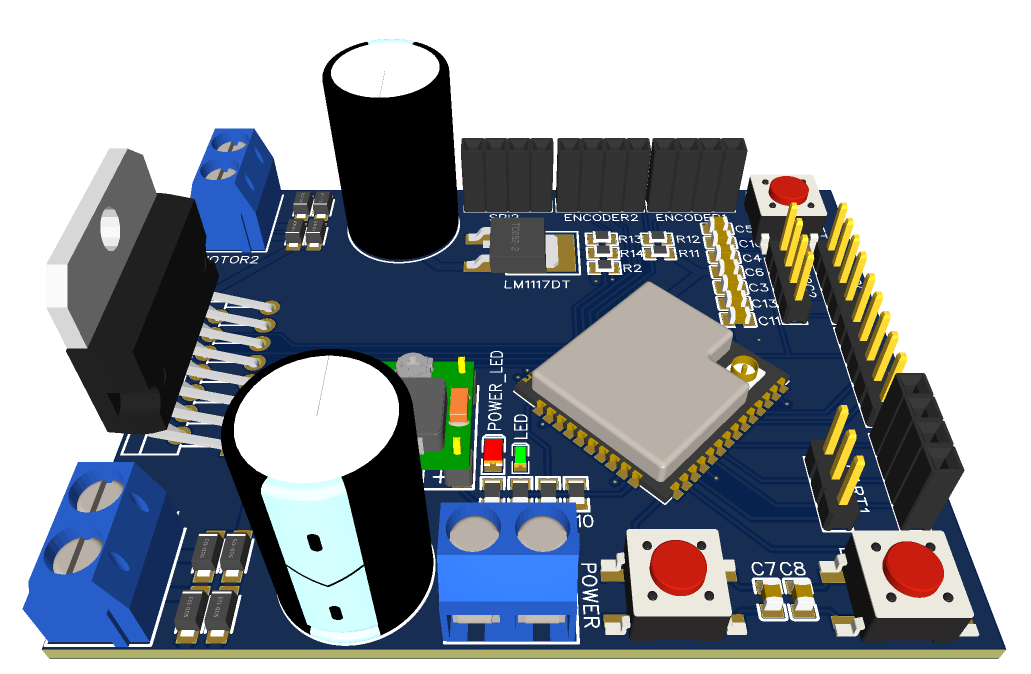
\includegraphics[height=0.32\textheight]{img/prototype_sym_1.png}
        \caption{Symulacja  gotowego urządzenia (wierzch)}
        \label{fig:prototype_sym_1}
    \end{figure}
    
    \begin{figure}[ht]
        \centering
        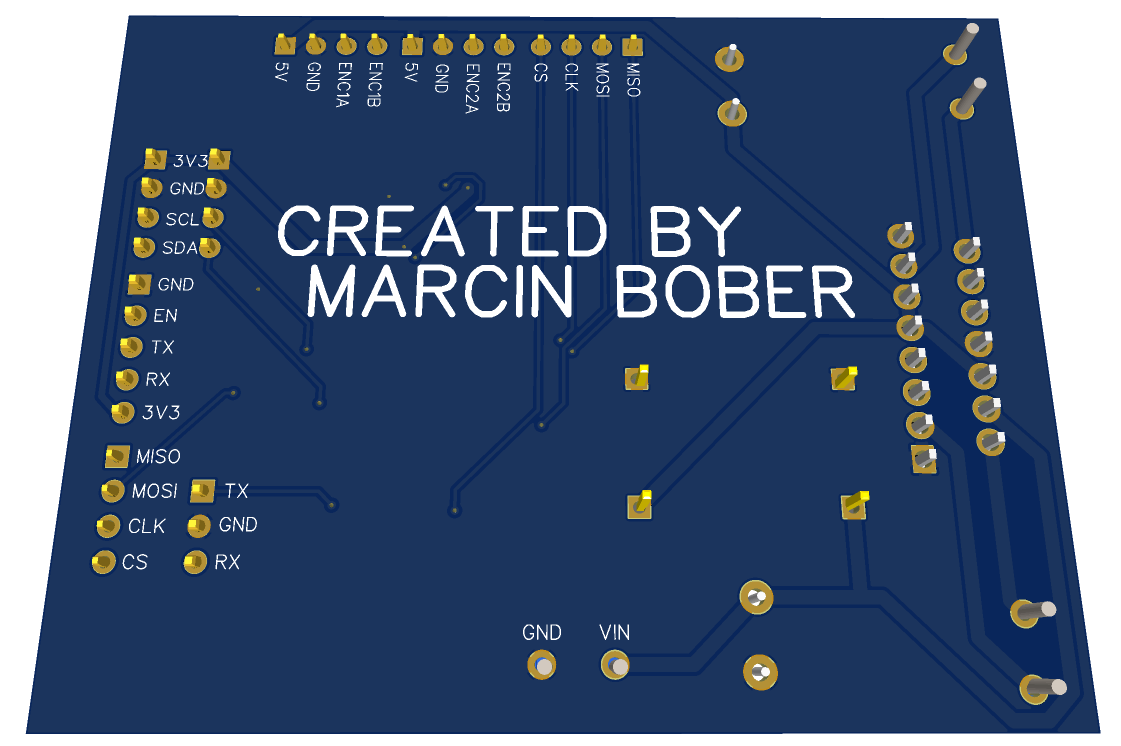
\includegraphics[height=0.32\textheight]{img/prototype_sym_2.png}
        \caption{Symulacja gotowego urządzenia (spód)}
        \label{fig:prototype_sym_2}
    \end{figure}

    
    \subsection{Prototyp}
    Zdjęcia  gotowego urządzenia zostały przedstawione na rysunkach \ref{fig:prototype_real_1} oraz \ref{fig:prototype_real_2}.
    
    \begin{figure}[ht]
        \centering
        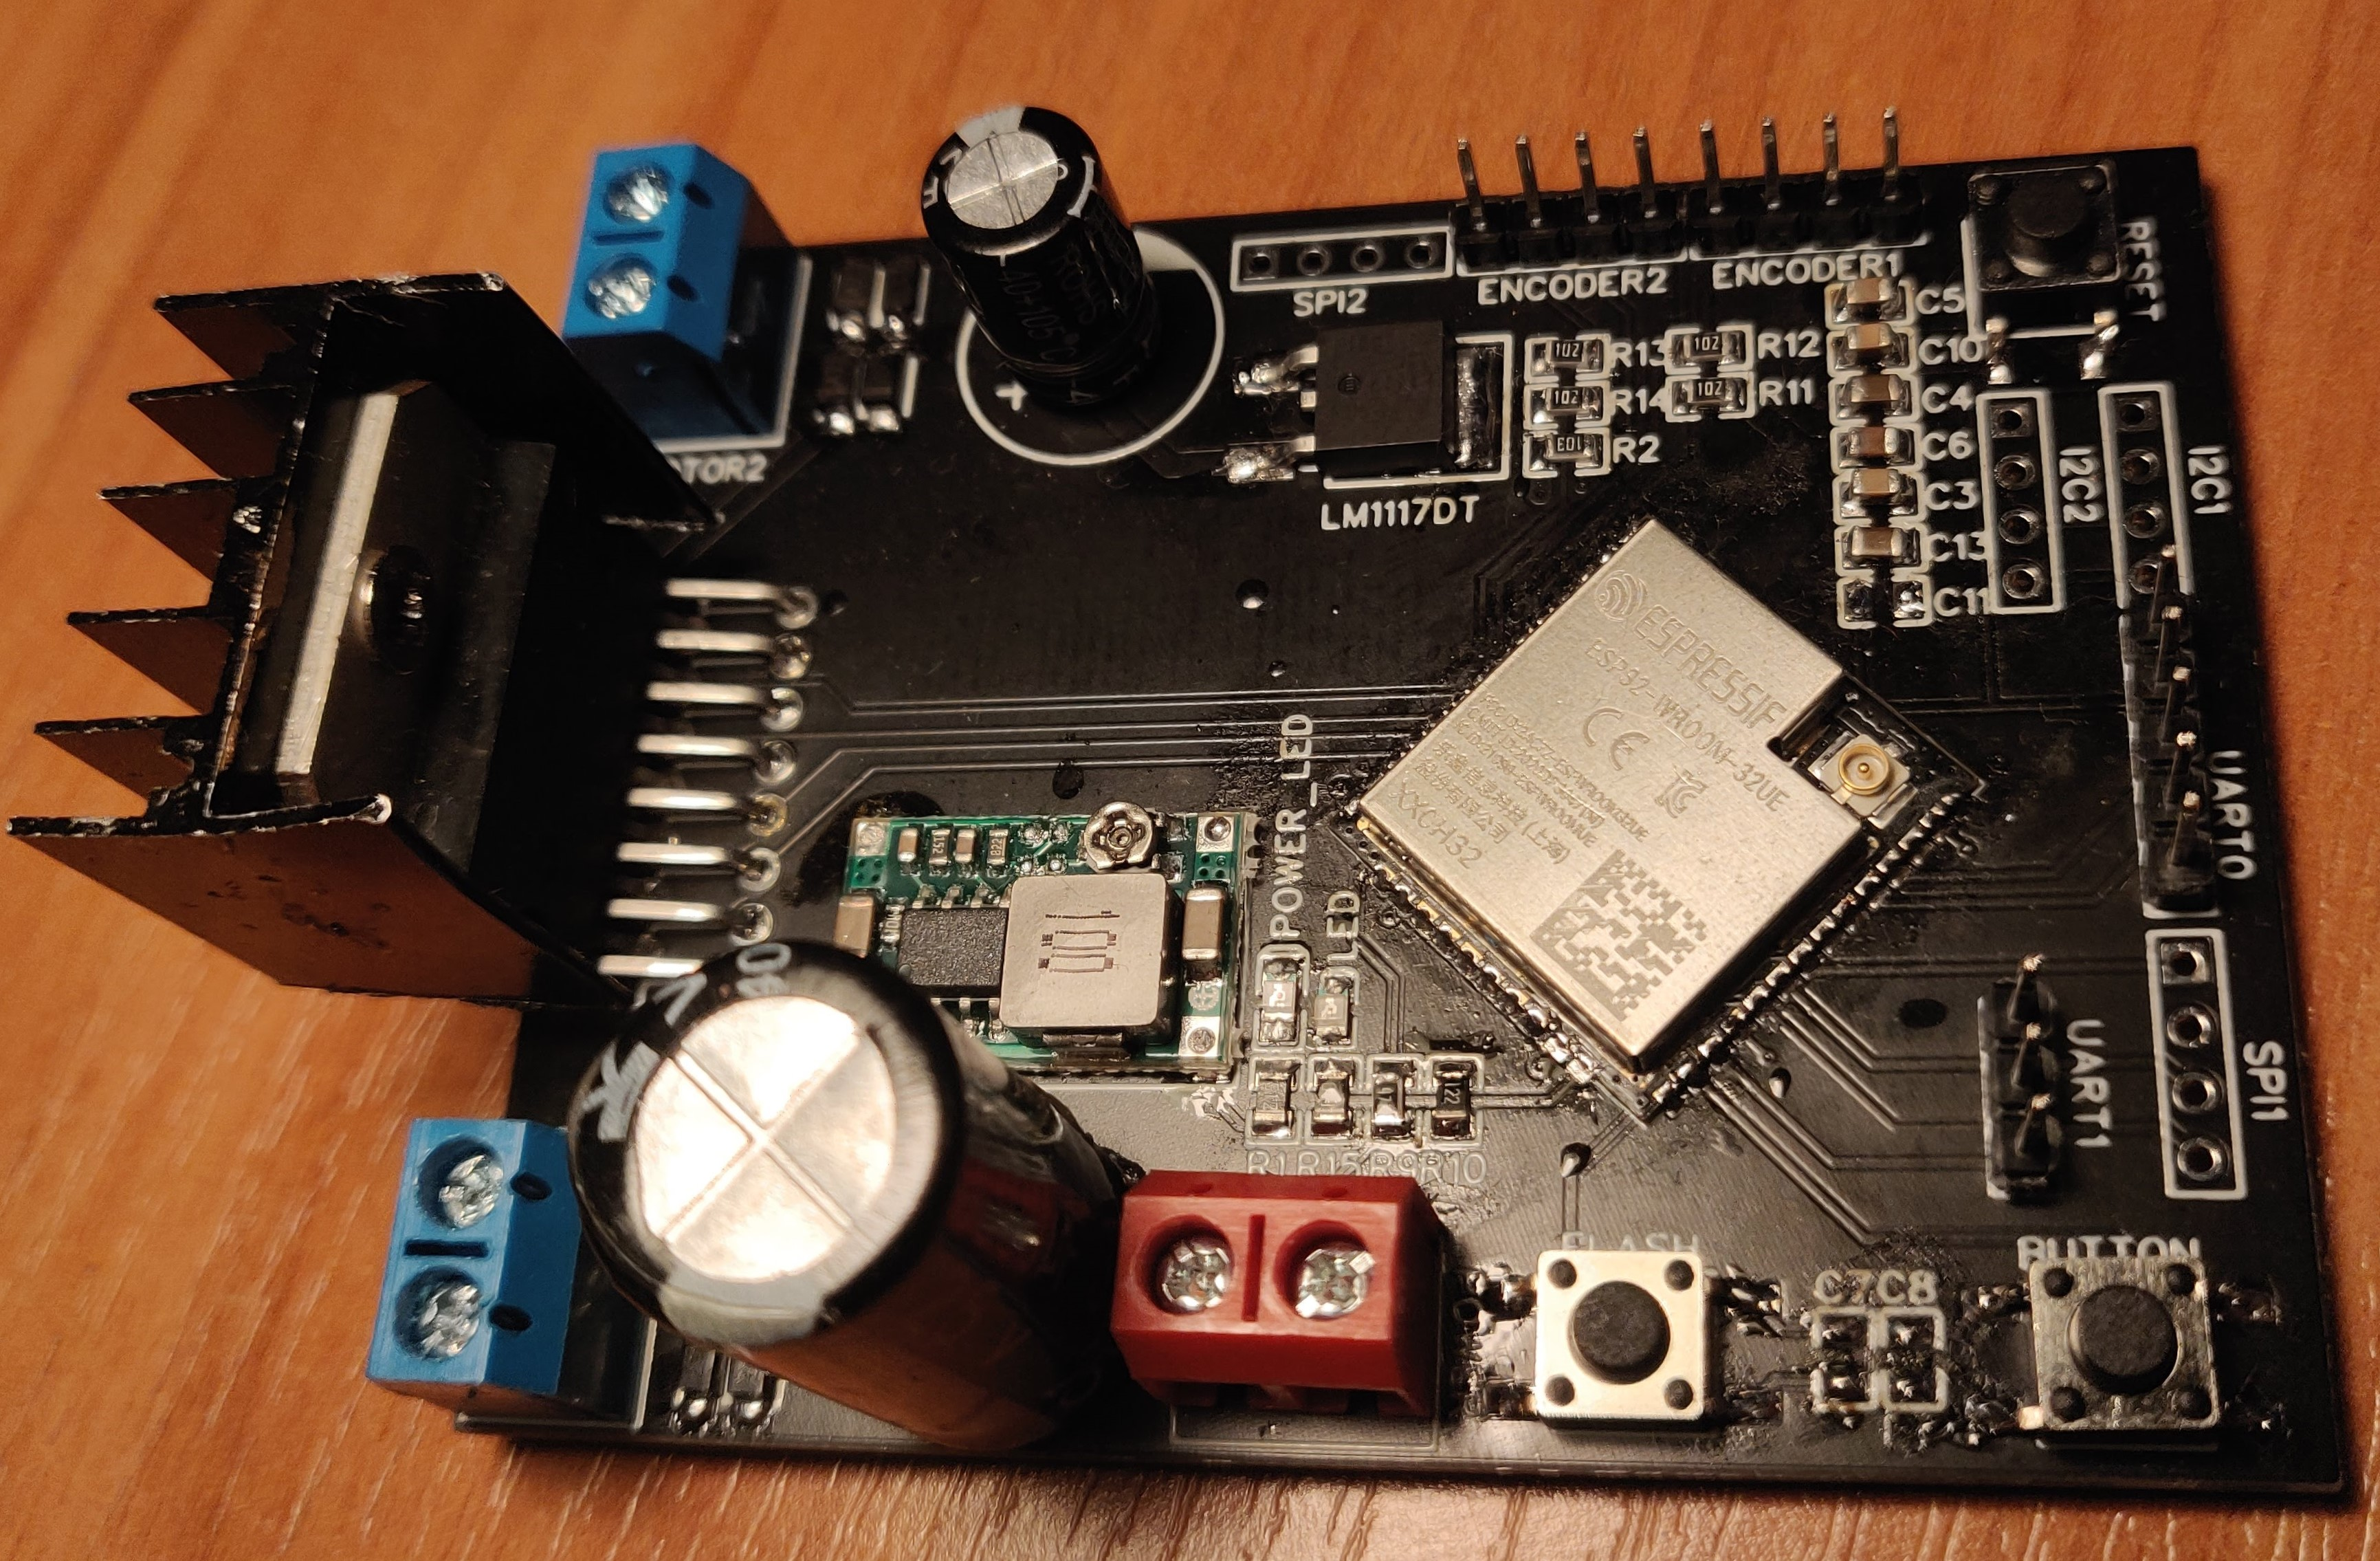
\includegraphics[height=0.4\textheight]{img/prototype_real_1.jpg}
        \caption{Zdjęcie gotowego urządzenia (wierzch)}
        \label{fig:prototype_real_1}
    \end{figure}
    
    \begin{figure}[ht]
        \centering
        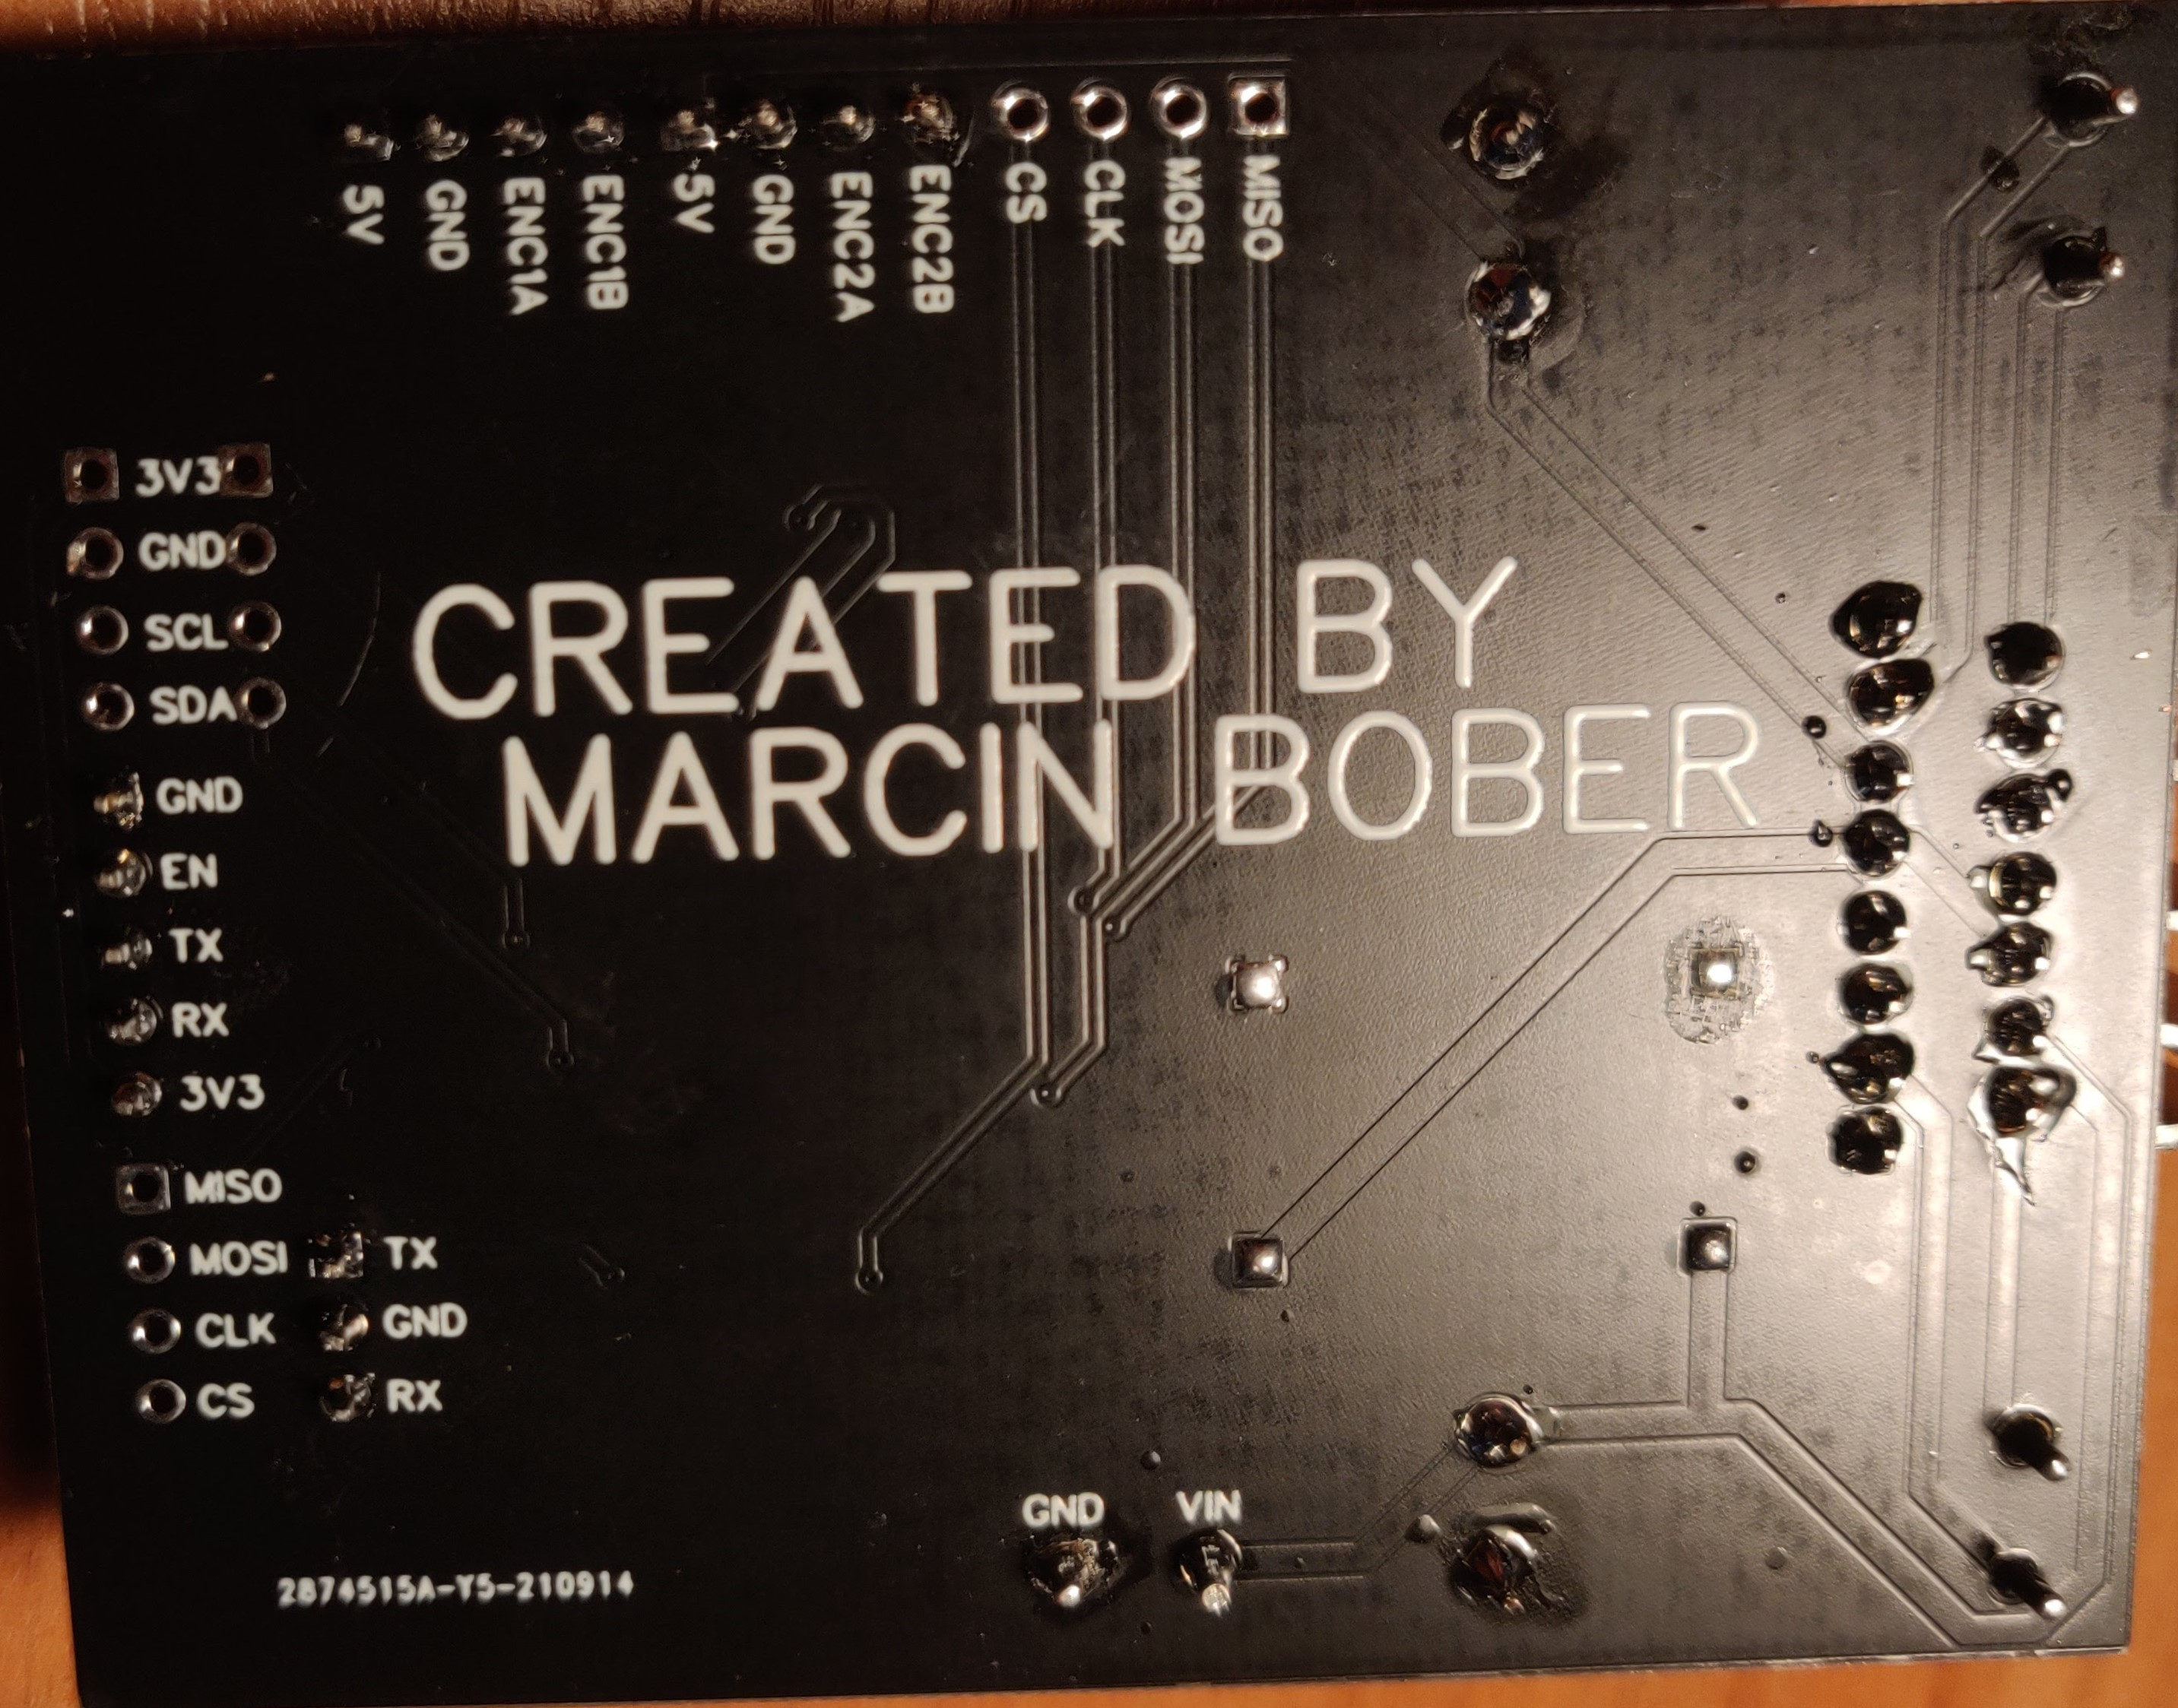
\includegraphics[height=0.45\textheight]{img/prototype_real_2.jpg}
        \caption{Zdjęcie gotowego urządzenia (spód)}
        \label{fig:prototype_real_2}
    \end{figure}